\documentclass[10pt]{article}
\usepackage[margin=0.55in,top=0.5in,bottom=0.5in]{geometry}
\usepackage[all]{xy}
\usepackage{caption}
\usepackage{amsmath,amsthm,amssymb,color,latexsym}
\usepackage{mathtools}
\usepackage{geometry}
\usepackage{booktabs}
\geometry{letterpaper}    
\usepackage{graphicx}
\usepackage{tabto}
\usepackage{setspace}
\usepackage[dvipsnames]{xcolor}
\usepackage[font=footnotesize]{caption}
\captionsetup{aboveskip=2pt, belowskip=2pt}
\setlength{\textfloatsep}{6pt plus 2pt minus 2pt}
\setlength{\floatsep}{6pt plus 2pt minus 2pt}
\setlength{\intextsep}{6pt plus 2pt minus 2pt}

\usepackage[noframe]{showframe}
\usepackage{framed}


\renewenvironment{shaded}{%
  \def\FrameCommand{\fboxsep=\FrameSep \colorbox{shadecolor}}%
  \MakeFramed{\advance\hsize-\width \FrameRestore\FrameRestore}}%
 {\endMakeFramed}
\definecolor{shadecolor}{gray}{0.90}

\newtheorem{problem}{Problem}

\newenvironment{solution}[1][\it{Solution:}]{\textbf{#1 } }

\singlespacing

\begin{document}
\graphicspath{{figures/}}

\begin{titlepage}
   \begin{center}
       \vspace*{9cm}

       \textbf{CS 332 Fall 2025}

       \vspace{0.5cm}
        Project \#4
        \vfill

       \textbf{Koshi Harashima, Ben Cole}\\
       Due Date: 11/19, 2025
            
   \end{center}
\end{titlepage}

\pagebreak

%%%%%%%%%%%%%%%%%%%%%%%%%%%%%%%%%%%%%%%%%%%%%%%%%%%%%%%%%%%
%%%%%%%%%%%%%%%%%%%%%%%% Problems %%%%%%%%%%%%%%%%%%%%%%%%%
%%%%%%%%%%%%%%%%%%%%%%%%%%%%%%%%%%%%%%%%%%%%%%%%%%%%%%%%%%%

%--------------------------------------------------------
% ===================== Add to preamble (after \usepackage{xcolor}) =====================
\usepackage[most]{tcolorbox}
\newtcolorbox{shaded}{
  colback=gray!10,
  colframe=gray!45,
  boxrule=0.6pt,
  arc=2mm,
  left=2mm,right=2mm,top=1.2mm,bottom=1.2mm
}

% ===================== Put this where you want the summary section =====================
% ---------------------- Part 1 ----------------------
\section{Outcomes (Part 1): Online Reserve Pricing}
\begin{shaded}
\textbf{Methods}\\
Repeated single-item second-price auctions with a reserve price $r$ over $T=20{,}000$ rounds. Each round has $m$ i.i.d.\ bidders with truthful bids (dominant strategy). Revenue is
\[
\mathrm{rev}=
\begin{cases}
0, & \max_i v_i < r,\\
\max\{r, v_{(2)}\}, & \text{otherwise,}
\end{cases}
\]
where $v_{(2)}$ is the second-highest value. We evaluate \emph{average revenue vs.\ time}, \emph{reserve trajectories}, and \emph{cumulative regret} against an (approximately) optimal fixed reserve computed by Monte Carlo grid search.\\[0.6em]

\textbf{Algorithms}\\
\emph{(i) Bandit baseline (epsilon-greedy)}: discretize reserves to a grid $\mathcal{G}\subset[0,1]$ with $|\mathcal{G}|=101$. Use exploration $\varepsilon_t=\min\{1,c/\sqrt{t}\}$; otherwise exploit the empirically best reserve.\\
\emph{(ii) Myerson plug-in (structure-aware)}: maintain an empirical CDF $\hat F$ from observed bids (full-information feedback under truthful bidding), and choose a reserve on a finer grid ($|\mathcal{G}|=1001$):
\[
r_t=\arg\max_{z\in\mathcal{G}} z\bigl(1-\hat F(z)\bigr).
\]
This exploits the monopoly-reserve structure that maximizes $r(1-F(r))$ under regularity.\\[0.6em]

\textbf{Results}\\
Across $F\in\{\mathrm{Uniform}[0,1],\; F(z)=z^2\}$ and bidder counts $m\in\{2,5,10\}$, both learners approach the Monte Carlo optimal fixed-reserve revenue. The plug-in method closes the gap earlier (lower early regret), and confidence intervals shrink over time. Higher $m$ increases revenue and accelerates stabilization (more informative order statistics each round). The Uniform $m{=}2$ case matches the analytic benchmark $r^\star=\tfrac12$ and $\mathbb{E}[\mathrm{rev}^\star]=\tfrac{5}{12}\approx0.4167$.\\[0.6em]

\textbf{Takeaways}\\
The plug-in method wins because it uses economic structure rather than treating reserves as unrelated arms. Generic bandits eventually work, but they waste rounds exploring dominated reserves. Market thickness ($m$) is not just ``more revenue''---it is strictly more information per round, so learning becomes easier.
\end{shaded}
\end{frame}

% ---------------------- Part 2 ----------------------
\section{Outcomes (Part 2): Online Revenue Maximization in Position Auctions}
\begin{shaded}
\textbf{Methods}\\
Position auction with click-through rates $w_1\ge \cdots \ge w_m$ and independent per-click values $v_i\sim F_i$ (allowing heterogeneity across bidders). We measure revenue using \emph{expected clicks} (to remove Bernoulli noise and isolate learning effects). We compare truthful baselines and online learners via \emph{average revenue vs.\ time}, \emph{95\% CIs}, and \emph{cumulative regret} relative to an oracle revenue benchmark.\\[0.6em]

\textbf{Algorithms}\\
\emph{(i) VCG (truthful, welfare-optimal)}: rank bidders by $v_i$, assign top values to top slots, and charge externality payments (efficient but not revenue-optimal).\\
\emph{(ii) Oracle Myerson (truthful, revenue-optimal)}: compute virtual values $\phi_i(v_i)$ from the true $F_i$, allocate to maximize $\sum_j w_j\,\phi_i(v_i)$ (excluding non-positive virtual values), and set payments via Myerson’s payment identity.\\
\emph{(iii) Empirical Myerson (plug-in learner)}: estimate each $F_i$ from observed values to get $\hat\phi_i$, then allocate by $\sum_j w_j\,\hat\phi_i(v_i)$. This aims to learn the optimal truthful mechanism by learning the components ($F_i$) that define it.\\
\emph{(iv) Menu auction (posted prices per slot)}: post a menu of $(\text{slot }j,\ \text{price }p_j)$ options. Bidders choose the utility-maximizing option (truthful with respect to the posted menu), and prices can be updated online. This is flexible and handles heterogeneity naturally, but generally targets a \emph{suboptimal} revenue benchmark relative to full Myerson.\\[0.6em]

\textbf{Results}\\
Empirical Myerson rapidly tracks the oracle Myerson revenue (fast convergence to the correct target when estimation stabilizes), while VCG stays below because it optimizes welfare rather than revenue. The menu approach is learnable and robust in heterogeneous settings, but converges more slowly and typically plateaus below oracle Myerson due to restricted expressiveness (posted-price menus). Regret grows sublinearly and CI bands tighten, indicating stabilization; increasing the number of bidders and strengthening top-slot weights raises revenue and speeds convergence.\\[0.6em]

\textbf{Takeaways}\\
If your goal is \emph{optimal} revenue, you must learn (or assume) the virtual-value structure---that is why the Myerson plug-in has the right target. If your goal is \emph{robust deployability} under heterogeneity and changing conditions, menus are a pragmatic compromise: simpler incentives and online updates, but a real efficiency/revenue tradeoff you cannot wish away.
\end{shaded}
\end{frame}
% =========================
% Drop-in collage for YOUR slides
% (Just change the paths inside \includegraphics)
% =========================

% ---------- Part 1: Images (2x2 + 1) ----------
\begin{frame}{Part 1: Key Plots (Overview)}
\centering
\newcommand{\imgH}{0.28\textheight} % tweak 0.26–0.30 if needed

% Row 1
\begin{minipage}[t]{0.48\textwidth}
  \centering
  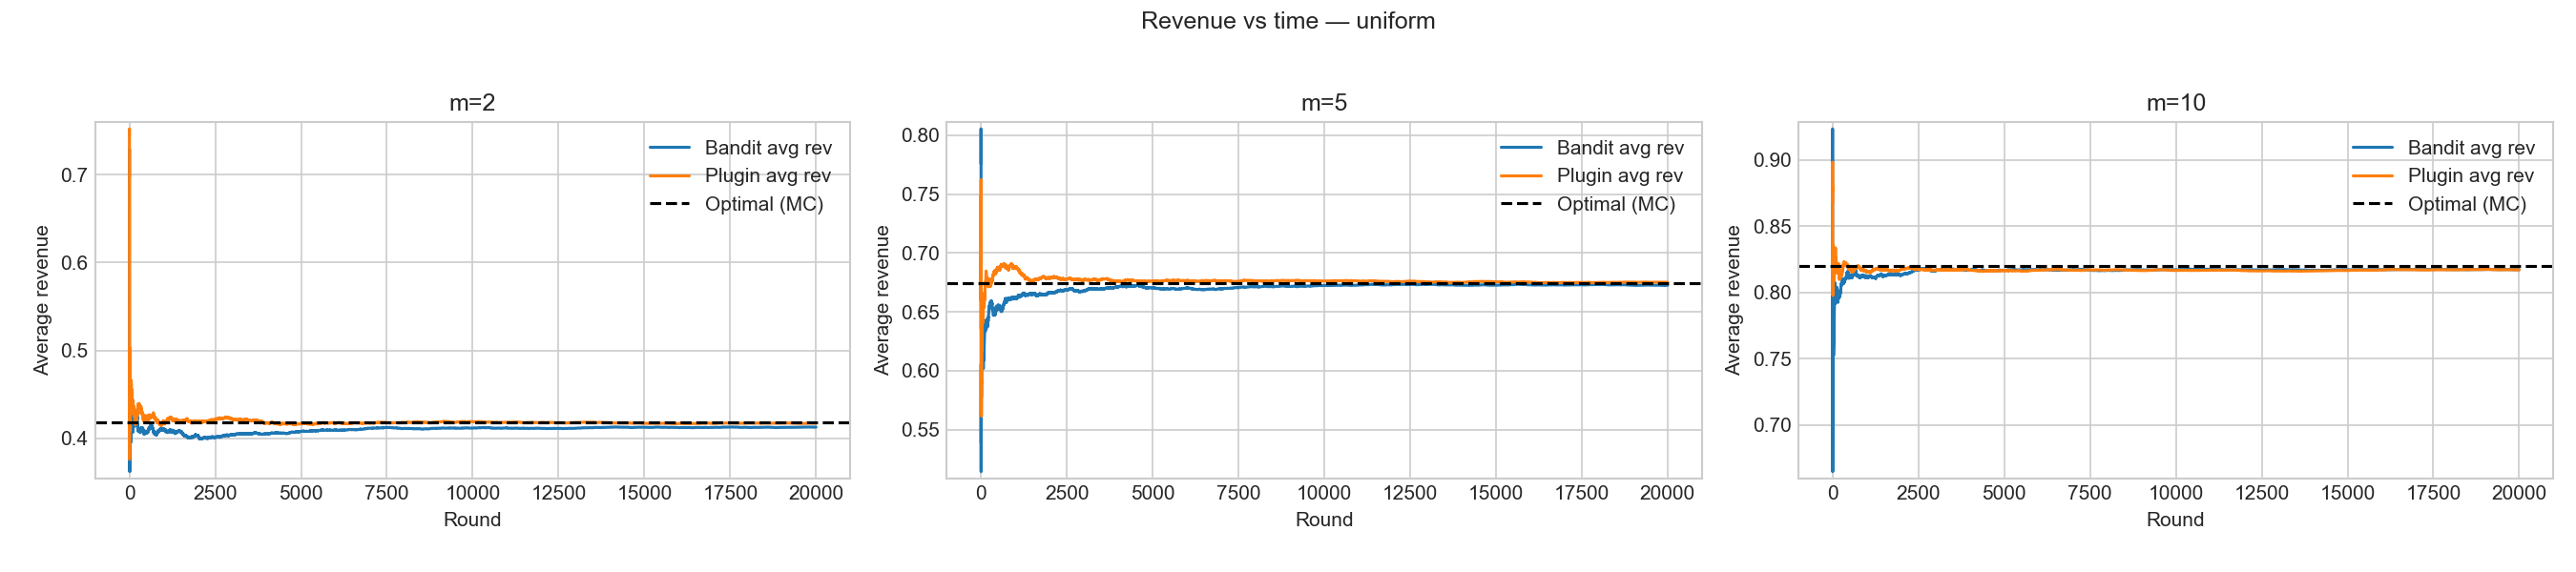
\includegraphics[width=\linewidth,height=\imgH,keepaspectratio]{part1/rev_uniform.png}
  \caption*{\footnotesize (1) Uniform — Revenue vs.\ time}
\end{minipage}\hfill
\begin{minipage}[t]{0.48\textwidth}
  \centering
  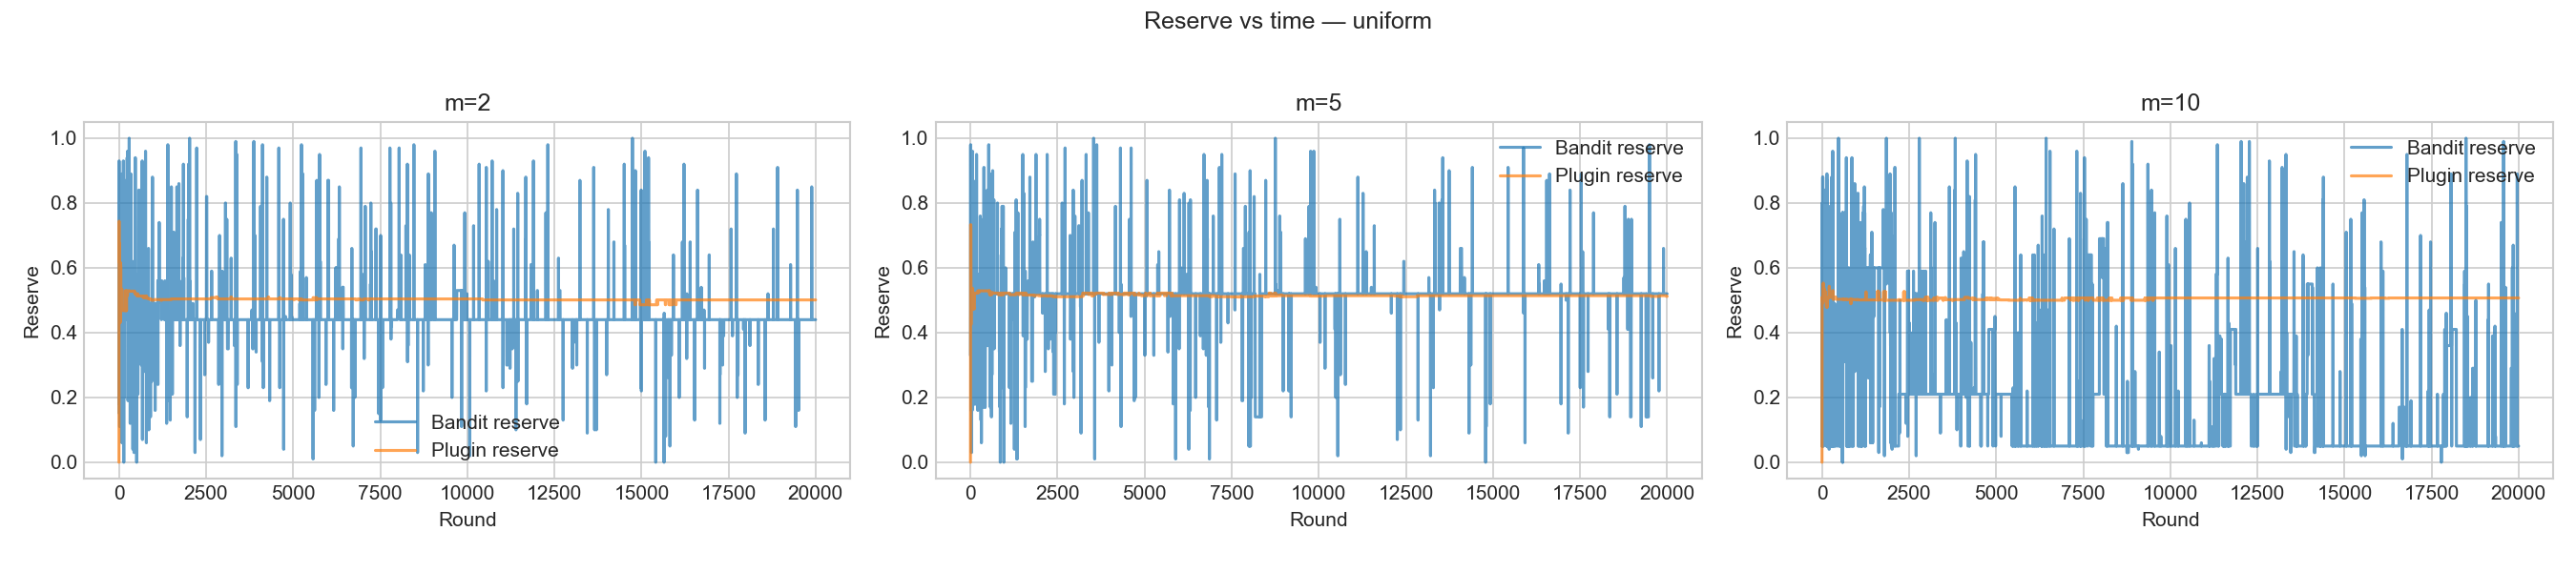
\includegraphics[width=\linewidth,height=\imgH,keepaspectratio]{part1/res_uniform.png}
  \caption*{\footnotesize (2) Uniform — Reserve trajectory}
\end{minipage}

\vspace{4pt}

% Row 2
\begin{minipage}[t]{0.48\textwidth}
  \centering
  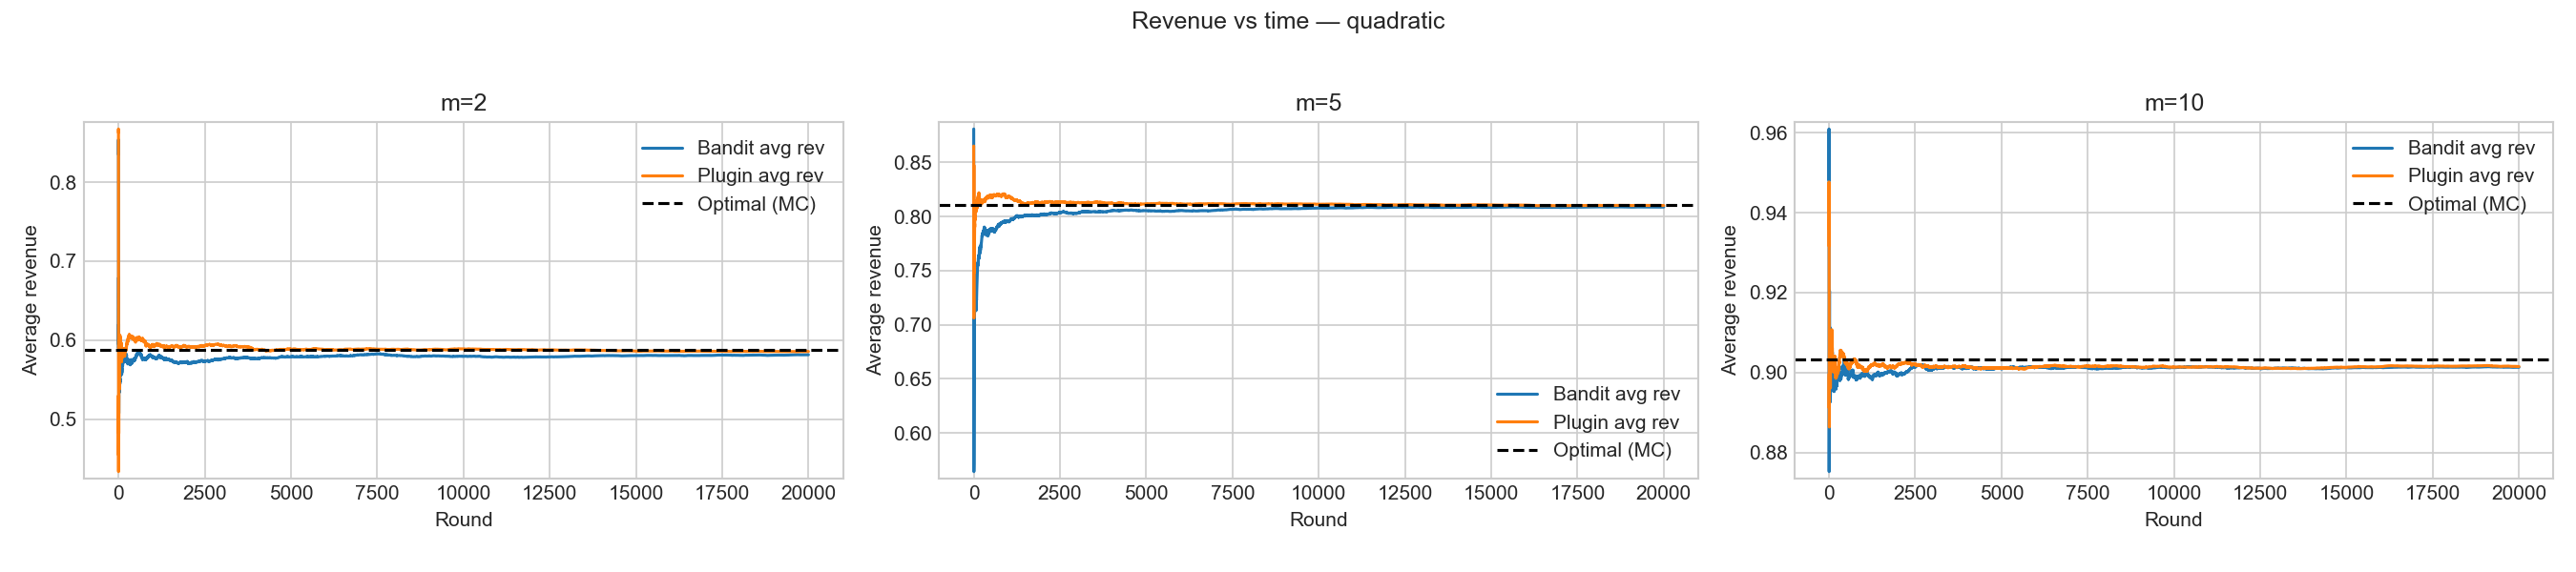
\includegraphics[width=\linewidth,height=\imgH,keepaspectratio]{part1/rev_quadratic.png}
  \caption*{\footnotesize (3) Quadratic $F(z)=z^2$ — Revenue vs.\ time}
\end{minipage}\hfill
\begin{minipage}[t]{0.48\textwidth}
  \centering
  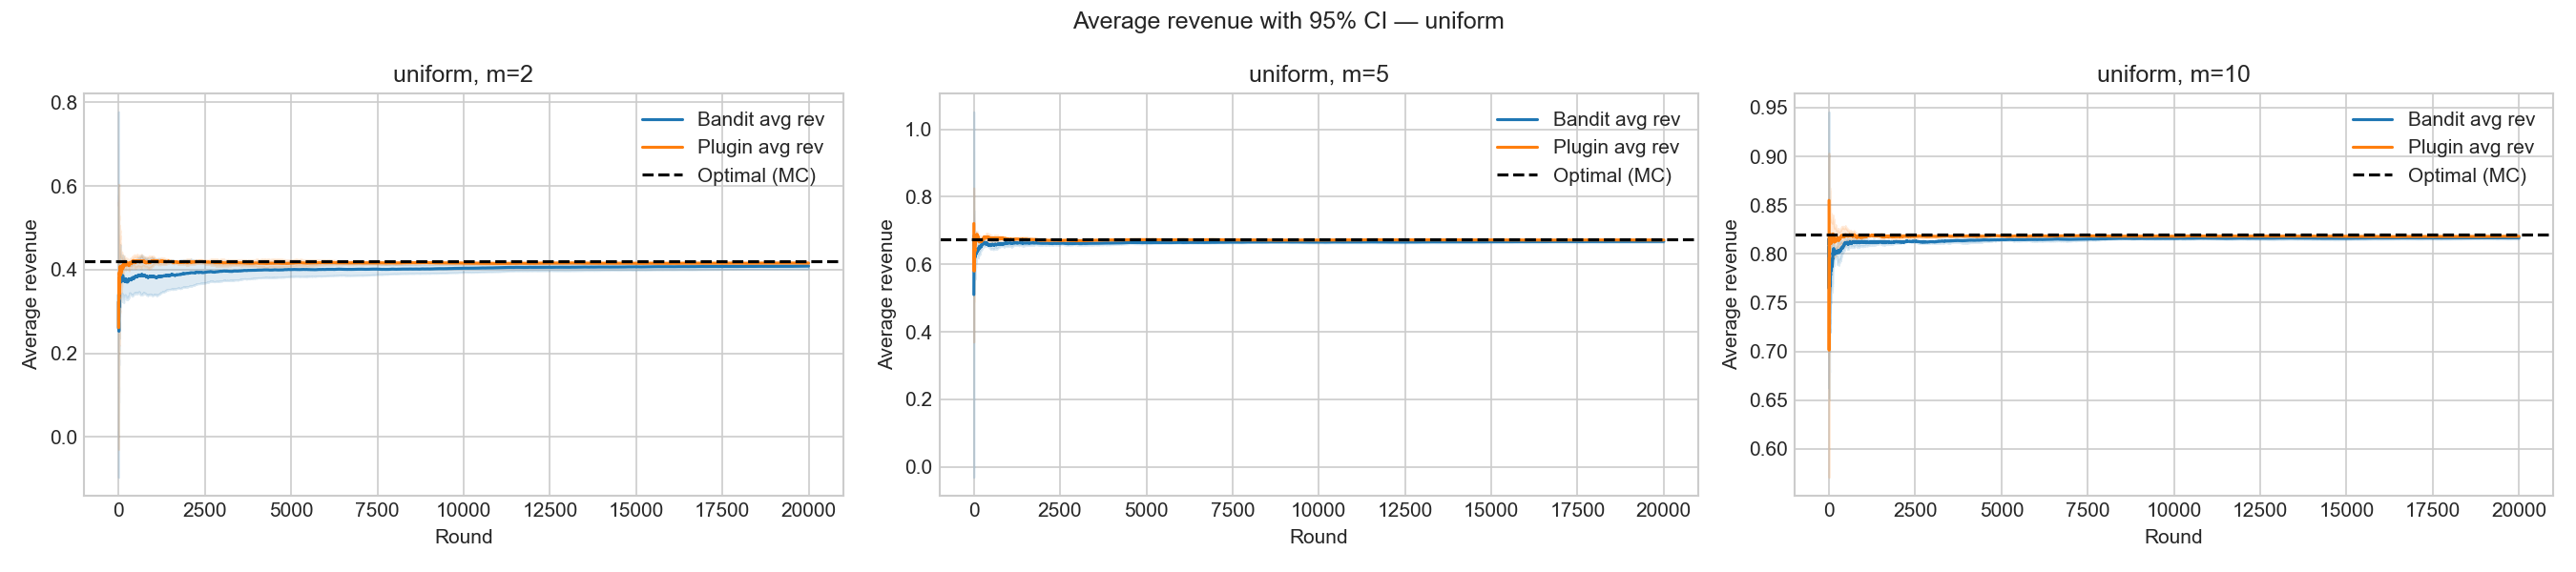
\includegraphics[width=\linewidth,height=\imgH,keepaspectratio]{part1/rev_uniform_ci.png}
  \caption*{\footnotesize (4) Uniform — Mean revenue with 95\% CI}
\end{minipage}

\vspace{4pt}

% Row 3 (single, centered)
\begin{minipage}[t]{0.70\textwidth}
  \centering
  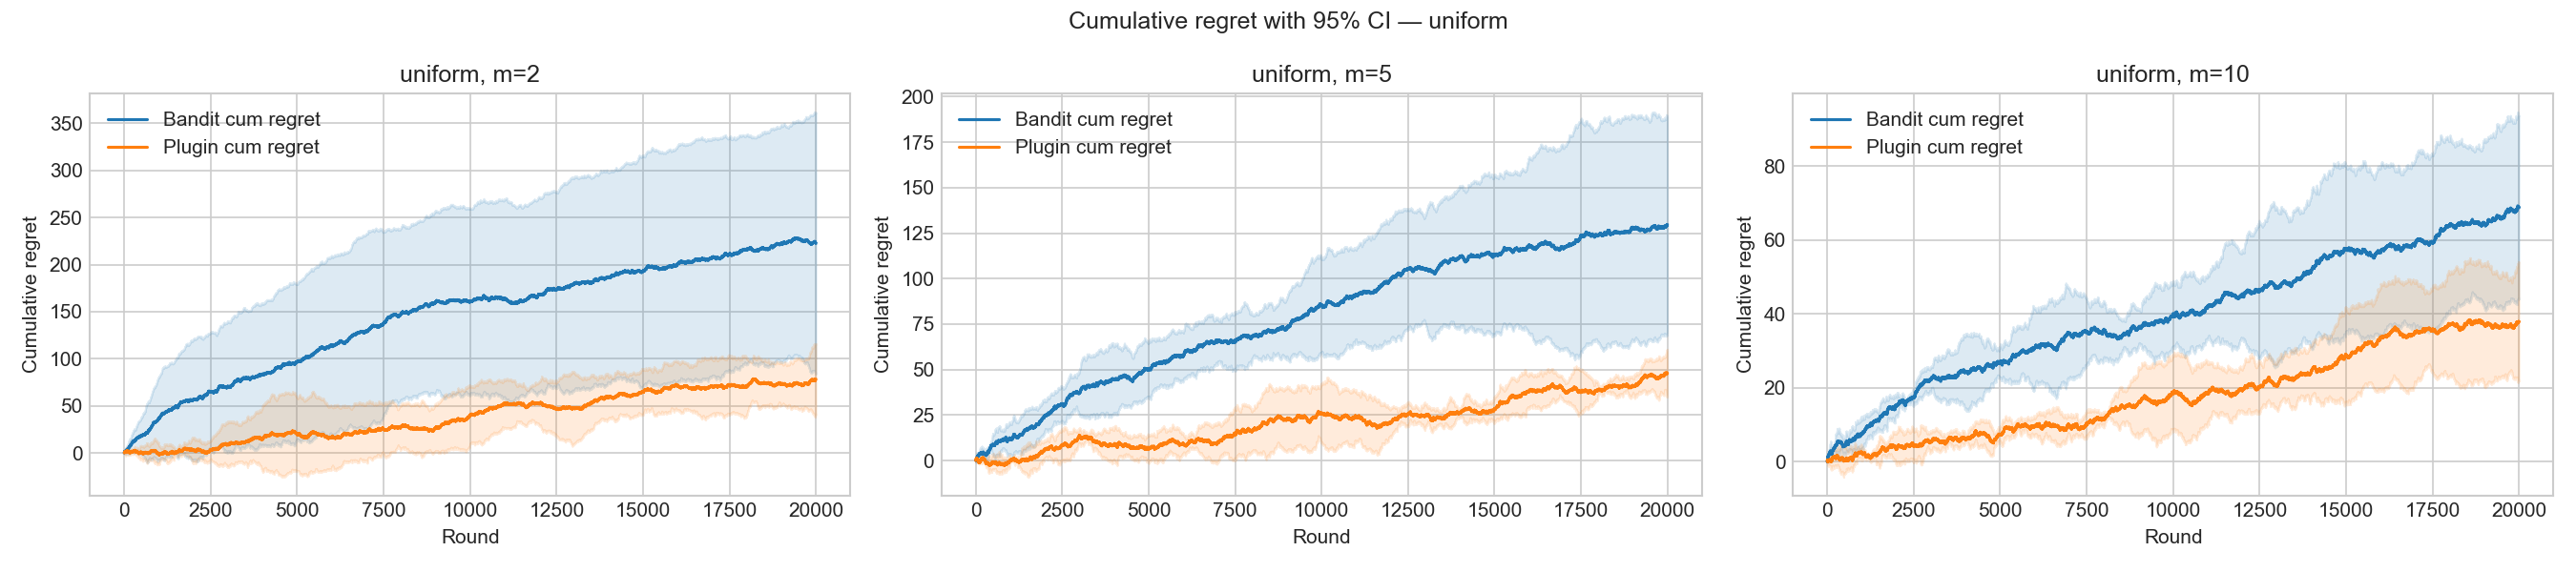
\includegraphics[width=\linewidth,height=0.24\textheight,keepaspectratio]{part1/regret_uniform_ci.png}
  \caption*{\footnotesize (5) Uniform — Cumulative regret with 95\% CI}
\end{minipage}
\end{frame}


% ---------- Part 1: Extra (Quadratic CI + Multi-unit) ----------
\begin{frame}{Part 1: Additional Evidence}
\centering
\newcommand{\imgH}{0.30\textheight} % tweak if needed

% Row 1
\begin{minipage}[t]{0.48\textwidth}
  \centering
  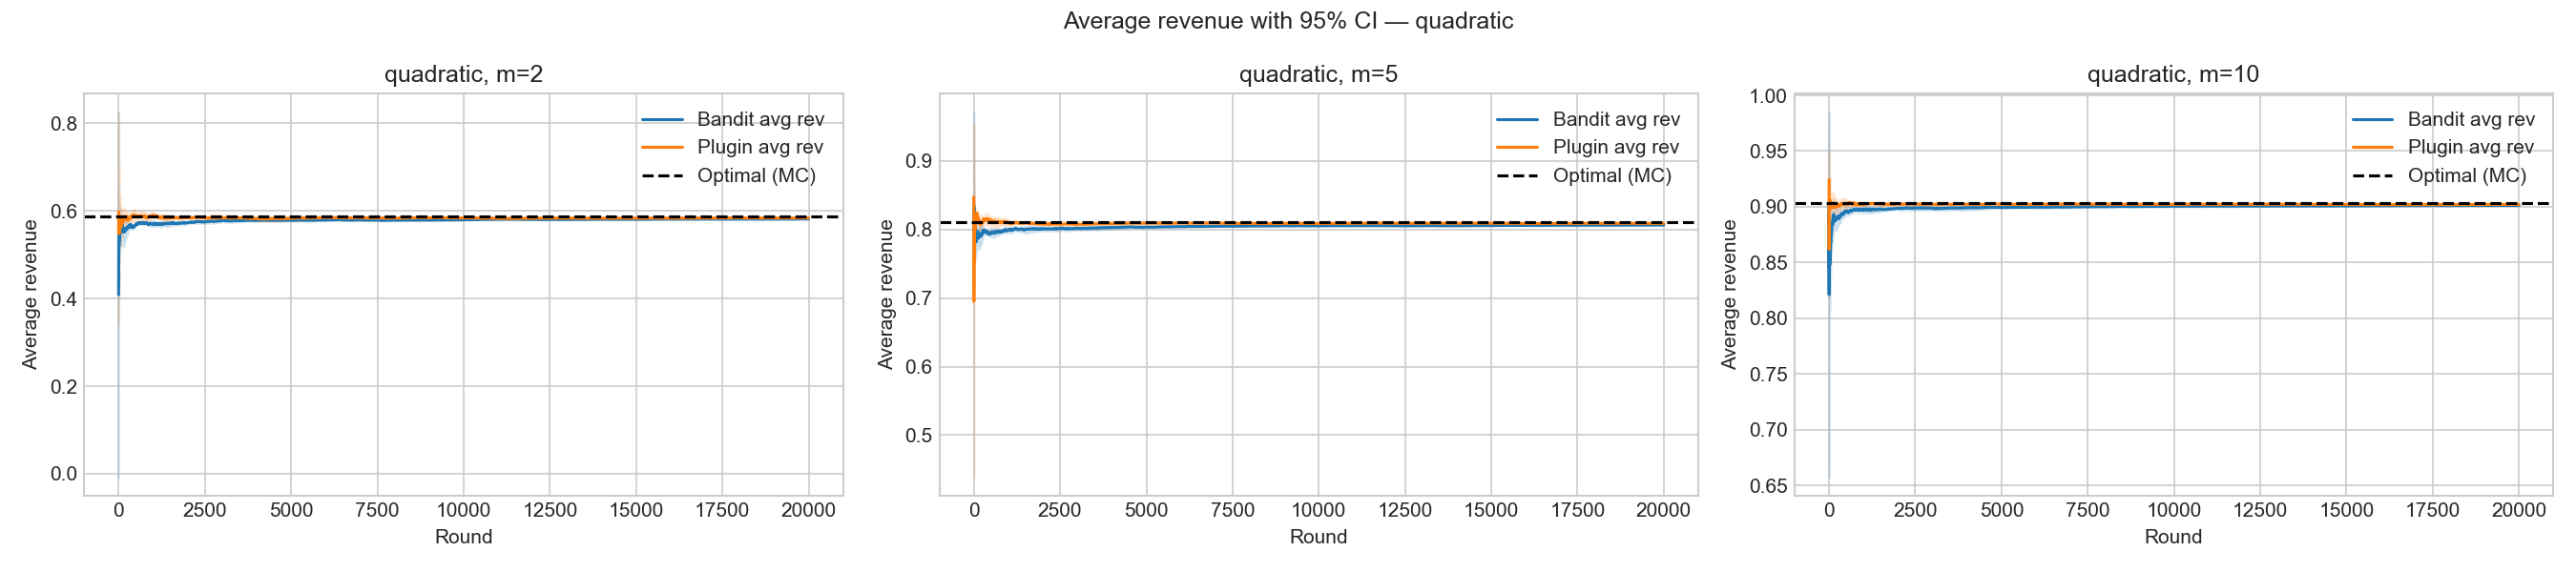
\includegraphics[width=\linewidth,height=\imgH,keepaspectratio]{part1/rev_quadratic_ci.png}
  \caption*{\footnotesize (1) Quadratic — Mean revenue with 95\% CI}
\end{minipage}\hfill
\begin{minipage}[t]{0.48\textwidth}
  \centering
  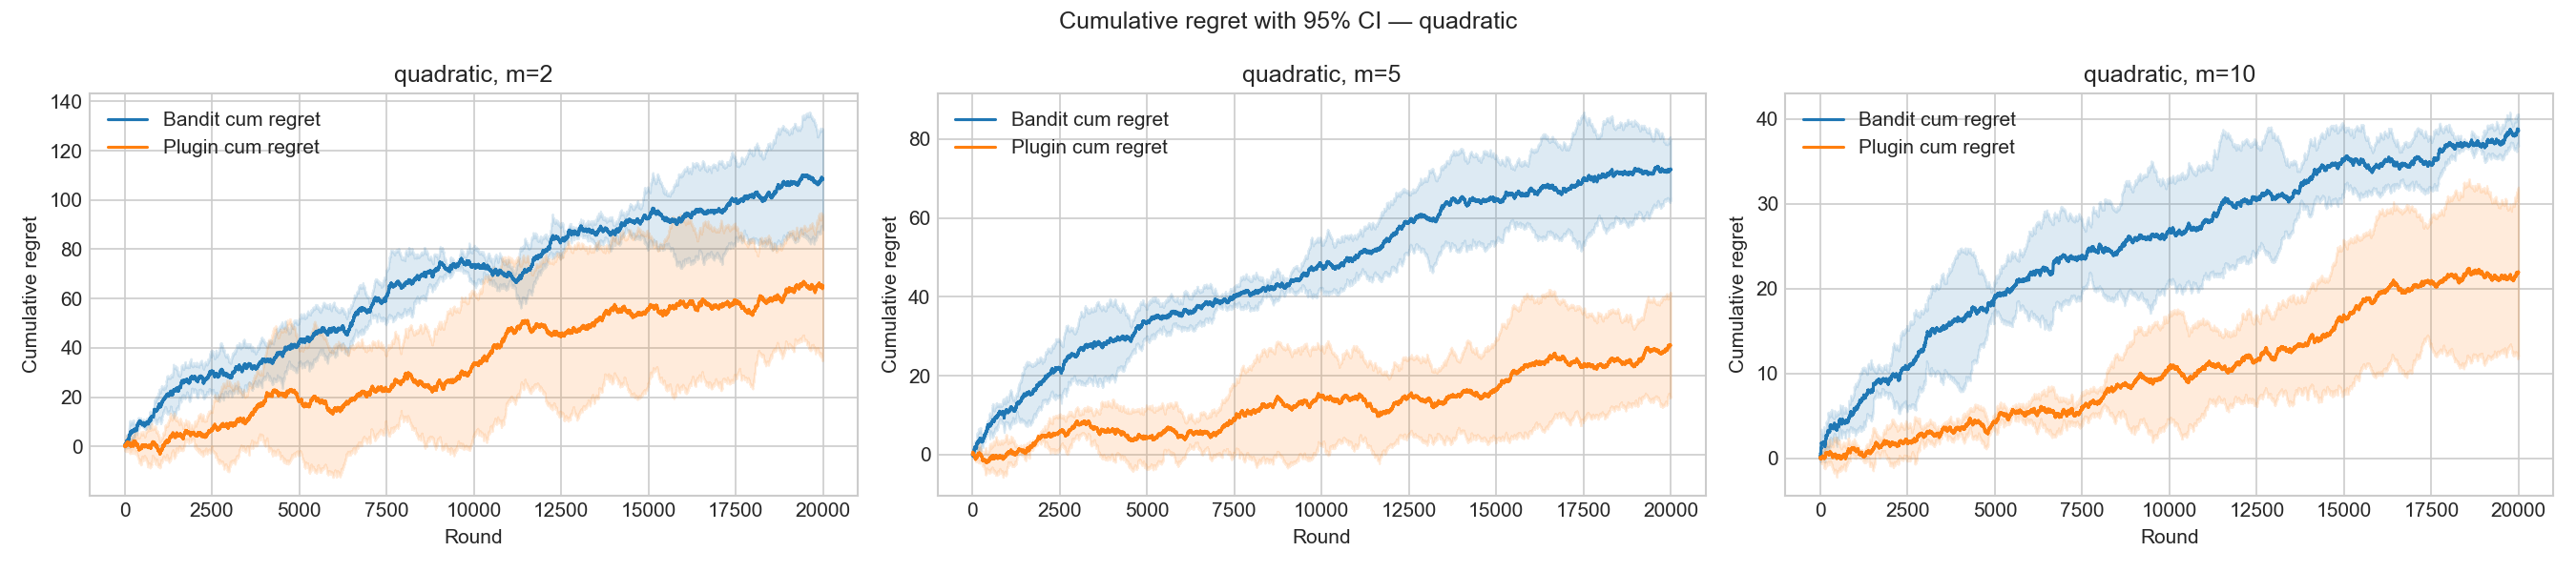
\includegraphics[width=\linewidth,height=\imgH,keepaspectratio]{part1/regret_quadratic_ci.png}
  \caption*{\footnotesize (2) Quadratic — Cumulative regret with 95\% CI}
\end{minipage}

\vspace{4pt}

% Row 2 (single, centered)
\begin{minipage}[t]{0.70\textwidth}
  \centering
  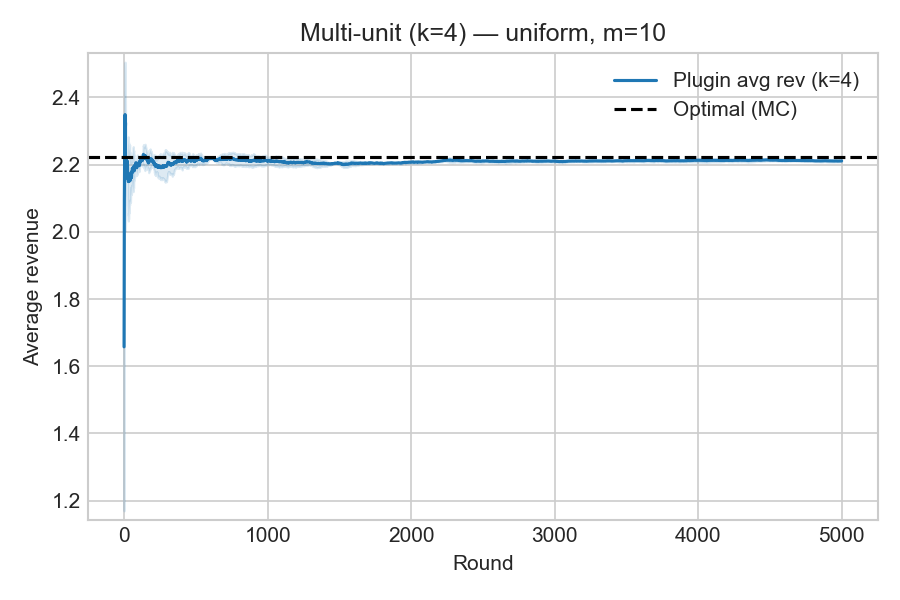
\includegraphics[width=\linewidth,height=0.28\textheight,keepaspectratio]{part1/rev_uniform_k4.png}
  \caption*{\footnotesize (3) Multi-unit ($k=4$) — Revenue vs.\ time}
\end{minipage}
\end{frame}


% ---------- Part 2: Images (2x2) ----------
\begin{frame}{Part 2: Key Plots (Overview)}
\centering
\newcommand{\imgH}{0.28\textheight} % tweak 0.26–0.30 if needed

% Row 1
\begin{minipage}[t]{0.48\textwidth}
  \centering
  
\includegraphics[width=\linewidth,height=\imgH,keepaspectratio]{332Project4/figures/part2/rev_uniform_menu_eg_ci.png}
  \caption*{\footnotesize (1) Uniform — Revenue (95\% CI)}
\end{minipage}\hfill
\begin{minipage}[t]{0.48\textwidth}
  \centering
  
\includegraphics[width=\linewidth,height=\imgH,keepaspectratio]{332Project4/figures/part2/regret_uniform_menu_eg_ci.png}
  \caption*{\footnotesize (2) Uniform — Regret (95\% CI)}
\end{minipage}

\vspace{4pt}

% Row 2
\begin{minipage}[t]{0.48\textwidth}
  \centering
  
\includegraphics[width=\linewidth,height=\imgH,keepaspectratio]{332Project4/figures/part2/rev_quadratic_menu_eg_ci.png}
  \caption*{\footnotesize (3) Quadratic — Revenue (95\% CI)}
\end{minipage}\hfill
\begin{minipage}[t]{0.48\textwidth}
  \centering
  
\includegraphics[width=\linewidth,height=\imgH,keepaspectratio]{332Project4/figures/part2/regret_quadratic_menu_eg_ci.png}
  \caption*{\footnotesize (4) Quadratic — Regret (95\% CI)}
\end{minipage}
\end{frame}


% ---------- Part 2: Sweeps / Extension (1x2) ----------
\begin{frame}{Part 2: Sweeps and Extension}
\centering
\newcommand{\imgH}{0.32\textheight}

\begin{minipage}[t]{0.48\textwidth}
  \centering
  
\includegraphics[width=\linewidth,height=\imgH,keepaspectratio]{332Project4/figures/part2/larger_m.png}
  \caption*{\footnotesize (1) Sweep — Larger $m$}
\end{minipage}\hfill
\begin{minipage}[t]{0.48\textwidth}
  \centering
  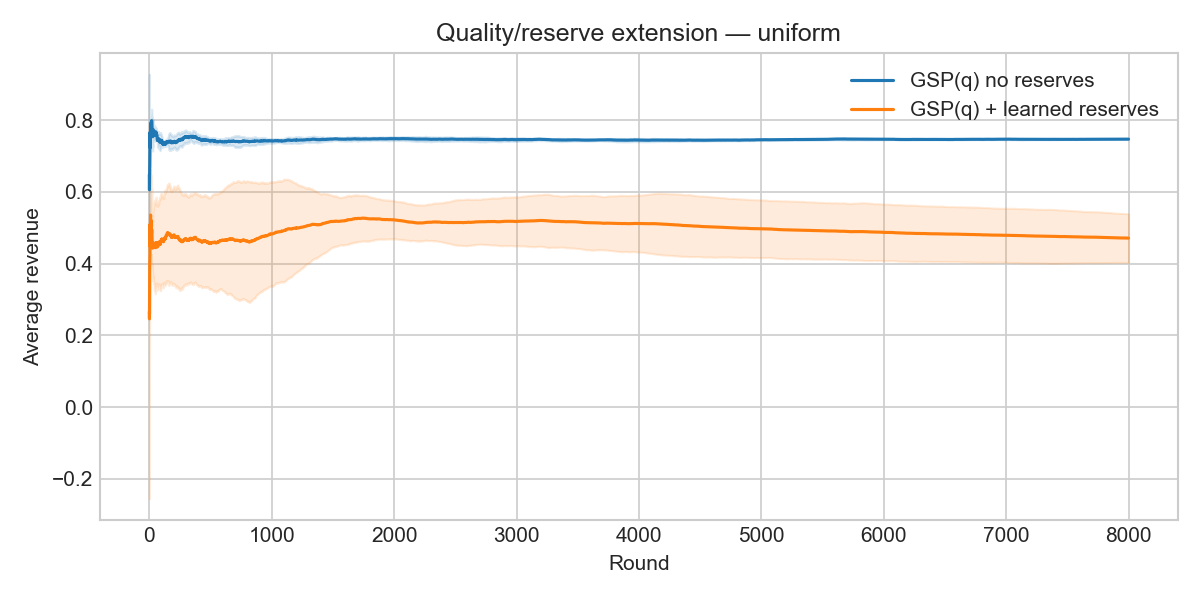
\includegraphics[width=\linewidth,height=\imgH,keepaspectratio]{figures/part2/ext_quality_reserves.png}
  \caption*{\footnotesize (2) Extension — Quality scores + slot reserves}
\end{minipage}
\end{frame}



\end{document}